% template created by: Russell Haering. arr. Joseph Crop
\documentclass[12pt]{article}
\usepackage[hmargin=1in, vmargin=1in]{geometry}
\usepackage{fancyhdr}
\pagestyle{fancy}
\usepackage[hang,small]{caption}
\usepackage{lastpage}
\usepackage{graphicx}
\usepackage{verbatim}
\DeclareGraphicsExtensions{.jpg}
\usepackage{url}

\def\author{Jacques Uber}
\def\title{ECE472 Lab1 Report}
\def\date{\today}

\fancyhf{} % clear all header and footer fields
\fancyhead[LO]{\author}
\fancyhead[RO]{\date}
% The weird spacing here is to get the spacing of \thepage to be right.
\fancyfoot[C]{\thepage\
                    / 7}

                    \setcounter{secnumdepth}{0}
                    \setlength{\parindent}{0pt}
                    \setlength{\parskip}{4mm}
                    \linespread{1.4}


\begin{document}
\fancyhf{} % clear all header and footer fields
\fancyhead[LO]{\author}
\fancyhead[RO]{\date}
\fancyhead[CO]{\title}



\section{Lab Report}
\begin{enumerate}
    \item
    Collect your waveform timing diagram for the circuit along with your
    finished, correct Verilog  code into one document. Annotate your simulation
    diagrams with notes/labels to explain what is being tested.

    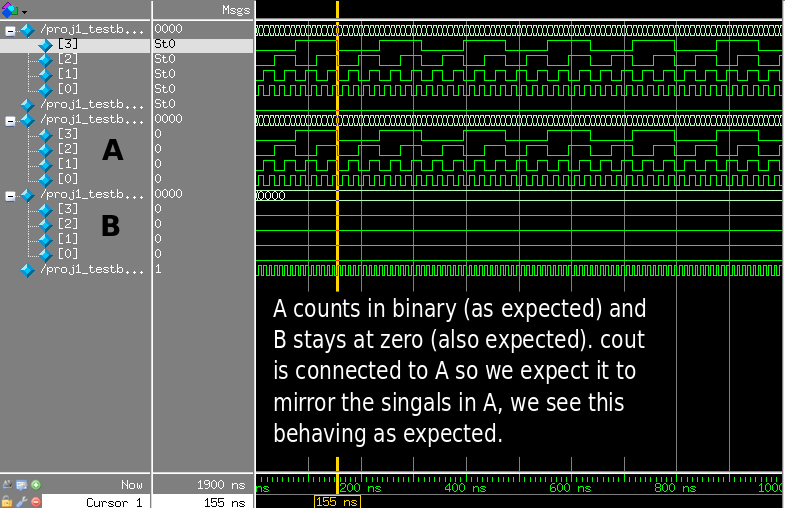
\includegraphics[scale=0.55]{wave.png}

    \item Lab Code
    {\tiny
    \begin{verbatim}
        module flipflop(reset, clk, d_in, d_out);
          input reset, clk;
          input d_in;
          output d_out;
          reg d_out;

          always @(posedge clk)
          begin

            if (reset)
              d_out <= 0;
            else
              d_out <= d_in;
          end
        endmodule

        module fulladder(a, b, cin, sum, cout);
            input a, b, cin;
            output sum, cout;

            assign sum = a ^ b ^ cin;
            assign cout = a & b | a & cin | b & cin;
        endmodule
        module mux(in_a, in_b, sel, out);
            input in_a, in_b;
            input sel;
            output out;
            reg out;

            always @(in_a or in_b or sel)
            begin
                case (sel)
                    1'b0: out = in_a;
                    1'b1: out = in_b;
                endcase
            end
        endmodule
        module ripple_adder(a, b, sum, cout);
            input [3:0] a, b;
            output [3:0] sum;
            output cout;

            wire [3:0] c;
            assign c[0]=0;

            fulladder f0(a[0], b[0], c[0], sum[0], c[1]);
            fulladder f1(a[1], b[1], c[1], sum[1], c[2]);
            fulladder f2(a[2], b[2], c[2], sum[2], c[3]);
            fulladder f3(a[3], b[3], c[3], sum[3], cout);
        endmodule
        module proj1_testbench;

            wire [3:0] sum;
            wire cout;

            reg [3:0] A, B;
            reg clk;

            // DUT = Device under test
            ripple_adder DUT(A, B, sum, cout);

            always
                #5 clk=~clk;

            initial begin
                clk = 1'b0;
                A = 8'h00;
                B = 8'h00;
            end

            always @(posedge clk)
            begin
                A = A + 1;
            end
        endmodule
    \end{verbatim}
    }

    \item
    Finally, indicate your estimate of the amount of time you spent on this project, what you  felt  was  most  valuable  and  least  valuable  about  this  project,  and  any suggestions you might have for improving this project in the future.

    I spent about 3 hours on this. I have never written any Verilog so most of the time I spent on this project was spent learning how to use and operate modelsim.

\end{enumerate}
\end{document}

